\subsection{La révolution des réseaux sociaux}
La communication a été théorisé par Claude Shannon en 1948 et a été portée par la suite aux sciences humaines.

Pour transmettre un message, il est nécessaire d'avoir deux entités : l'émetteur et le récepteur. Actuellement, le département prend le rôle d'émetteur tandis que les élèves et étudiants recherchant une formation prennent eux le rôle de récepteur. Ce mode de transmission de l'information est le plus couramment utilisé par le département ASI et l'INSA de Rouen, par exemple en distribuant des dépliants publicitaires.

\begin{center}
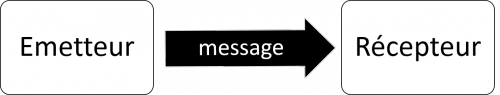
\includegraphics[scale=0.5]{./image/information.png}
\end{center}

L'étape suivant l'information est la communication. Le processus est similaire, mais cette fois, le récepteur renvois un message vers l'émetteur : une réaction, une question. C'est ce retour qui valide si le processus de communication est efficace. La communication est notamment utilisée lors des salons, des présentations, quand des ambassadeurs de l'INSA se déplace vers le publique destinataire.

\begin{center}
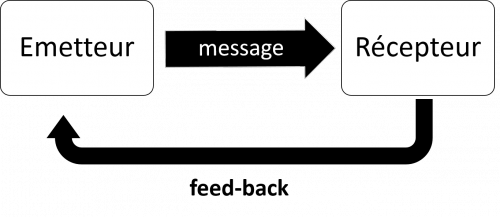
\includegraphics[scale=0.5]{./image/communication.png}
\end{center}

Avec l'arrivée des réseaux sociaux, la tendance s'est inversée. Ce n'est plus l'émetteur original mais le récepteur qui envois le message. Sur la page, mur, blog, fil d'actualité, ce n'est plus l'émetteur qui envois des messages, mais sa communauté. L'émetteur se doit alors de répondre, transmettre l'information, les messages et commentaire de sa communauté.

\begin{center}
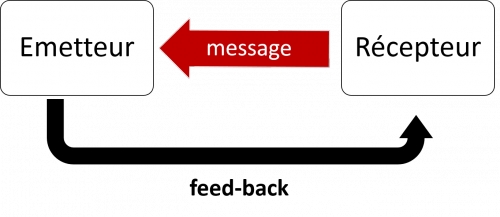
\includegraphics[scale=0.5]{./image/communication_digitale.png}
\end{center}

\subsection{Le métier de community manager}

\paragraph{}
Du fait de l'essor de ces nouveaux réseaux sociaux, de nouveaux métiers se sont également développés, 
très liés à ces médias et au web 2.0. Nous allons nous intéresser ici à un de ces métiers en particulier, 
que nous allons devoir pratiquer pendant quelques temps : celui de \emph{Community Manager}.

\paragraph{}
L'objectif premier du gestionnaire de communauté est d'interagir avec les membres d'une communauté d'une 
entité, que ce soit une entreprise, un événement, une groupe de musique ou, dans notre cas, un département 
d'école d'ingénieurs. Pour cela, il maîtrise tous les nouveaux médias du web tels que YouTube, Twitter, 
Facebook, etc. Le community manager est donc toujours au point sur les nouvelles technologies, les nouvelles 
plateformes de communication, sait repérer celles qui peuvent servir à la bonne réussite de sa mission. 

\paragraph{}
Il sait donc parfaitement comment susciter l'intérêt et les réactions de la communauté, quels contenus fournir 
aux différentes plateformes qu'il utilise pour les rendre dynamiques et attractives, et faire en sorte que la 
communauté reste fidèle, réactive et croissante.
Le community manager joue donc de multiples rôles : animateur, modérateur, fournisseur de contenu, dynamiseur, etc. 

\paragraph{}
Enfin, le saint Graal de tout community manager est le buzz. La vidéo YouTube à plusieurs millions de vues, 
le statut Facebook à plusieurs milliers de likes et partages, le Tweet retweeté sur toute la toile : le buzz 
peut provenir de n'importe quel média et peut permettre à une entreprise de consolider son image de marque - ou, 
au contraire, de la détruire. 

\subsection{Présence du public ciblé sur les réseaux sociaux}
En France, 68 \% des français sont inscrit sur au moins un réseau social. Les trois réseaux sociaux préférés des français sont Facebook (43\% des français l'utilise mensuellement), Google+ (11\%) et Twitter (10\%).

\subsubsection{Twitter}
Sur Twitter, seul 25\% des inscrits sont effectivement actifs et la communauté française compte seulement 2.3 millions d'utilisateurs (5\% des plus de 15 ans alors que 9 personnes sur 10 connaissent effectivement Twitter).
En France, l'âge moyen des utilisateur est de 22 ans, et 53\% d'entre eux sont des adolescents. De plus, un tiers des utilisateurs de Twitter habite l'île de France, région voisine de la Haute-Normandie. Le taux de pénétration du marché de Twitter est de seulement 4\%.

\subsubsection{Facebook}
Facebook est le réseaux social numéro 1 avec plus de 26 millions d'utilisateurs mensuel en France dont 18 millions quotidiennement. Un quart des utilisateurs a entre 18 et 24 ans et 16\% ont entre 13 et 17 ans. L'âge moyen des utilisateur est aussi de 22 ans.
Les pages les plus populaires sont Nutella, Coca-Cola, Oasis Be Fruit et M\&M's France. 

\subsubsection{Google+}
Il semblerait que Google+ soit un réseau social boudé par les français, qui ne compte que 40 000 actifs en france et un total de 83\% de compte inactif.
